\documentclass{standalone}
\usepackage{tikz}
\usetikzlibrary{patterns, positioning}
\usepackage[sfdefault]{ClearSans} %% option 'sfdefault' activates Clear Sans as the default text font
\usepackage[T1]{fontenc}

\begin{document}
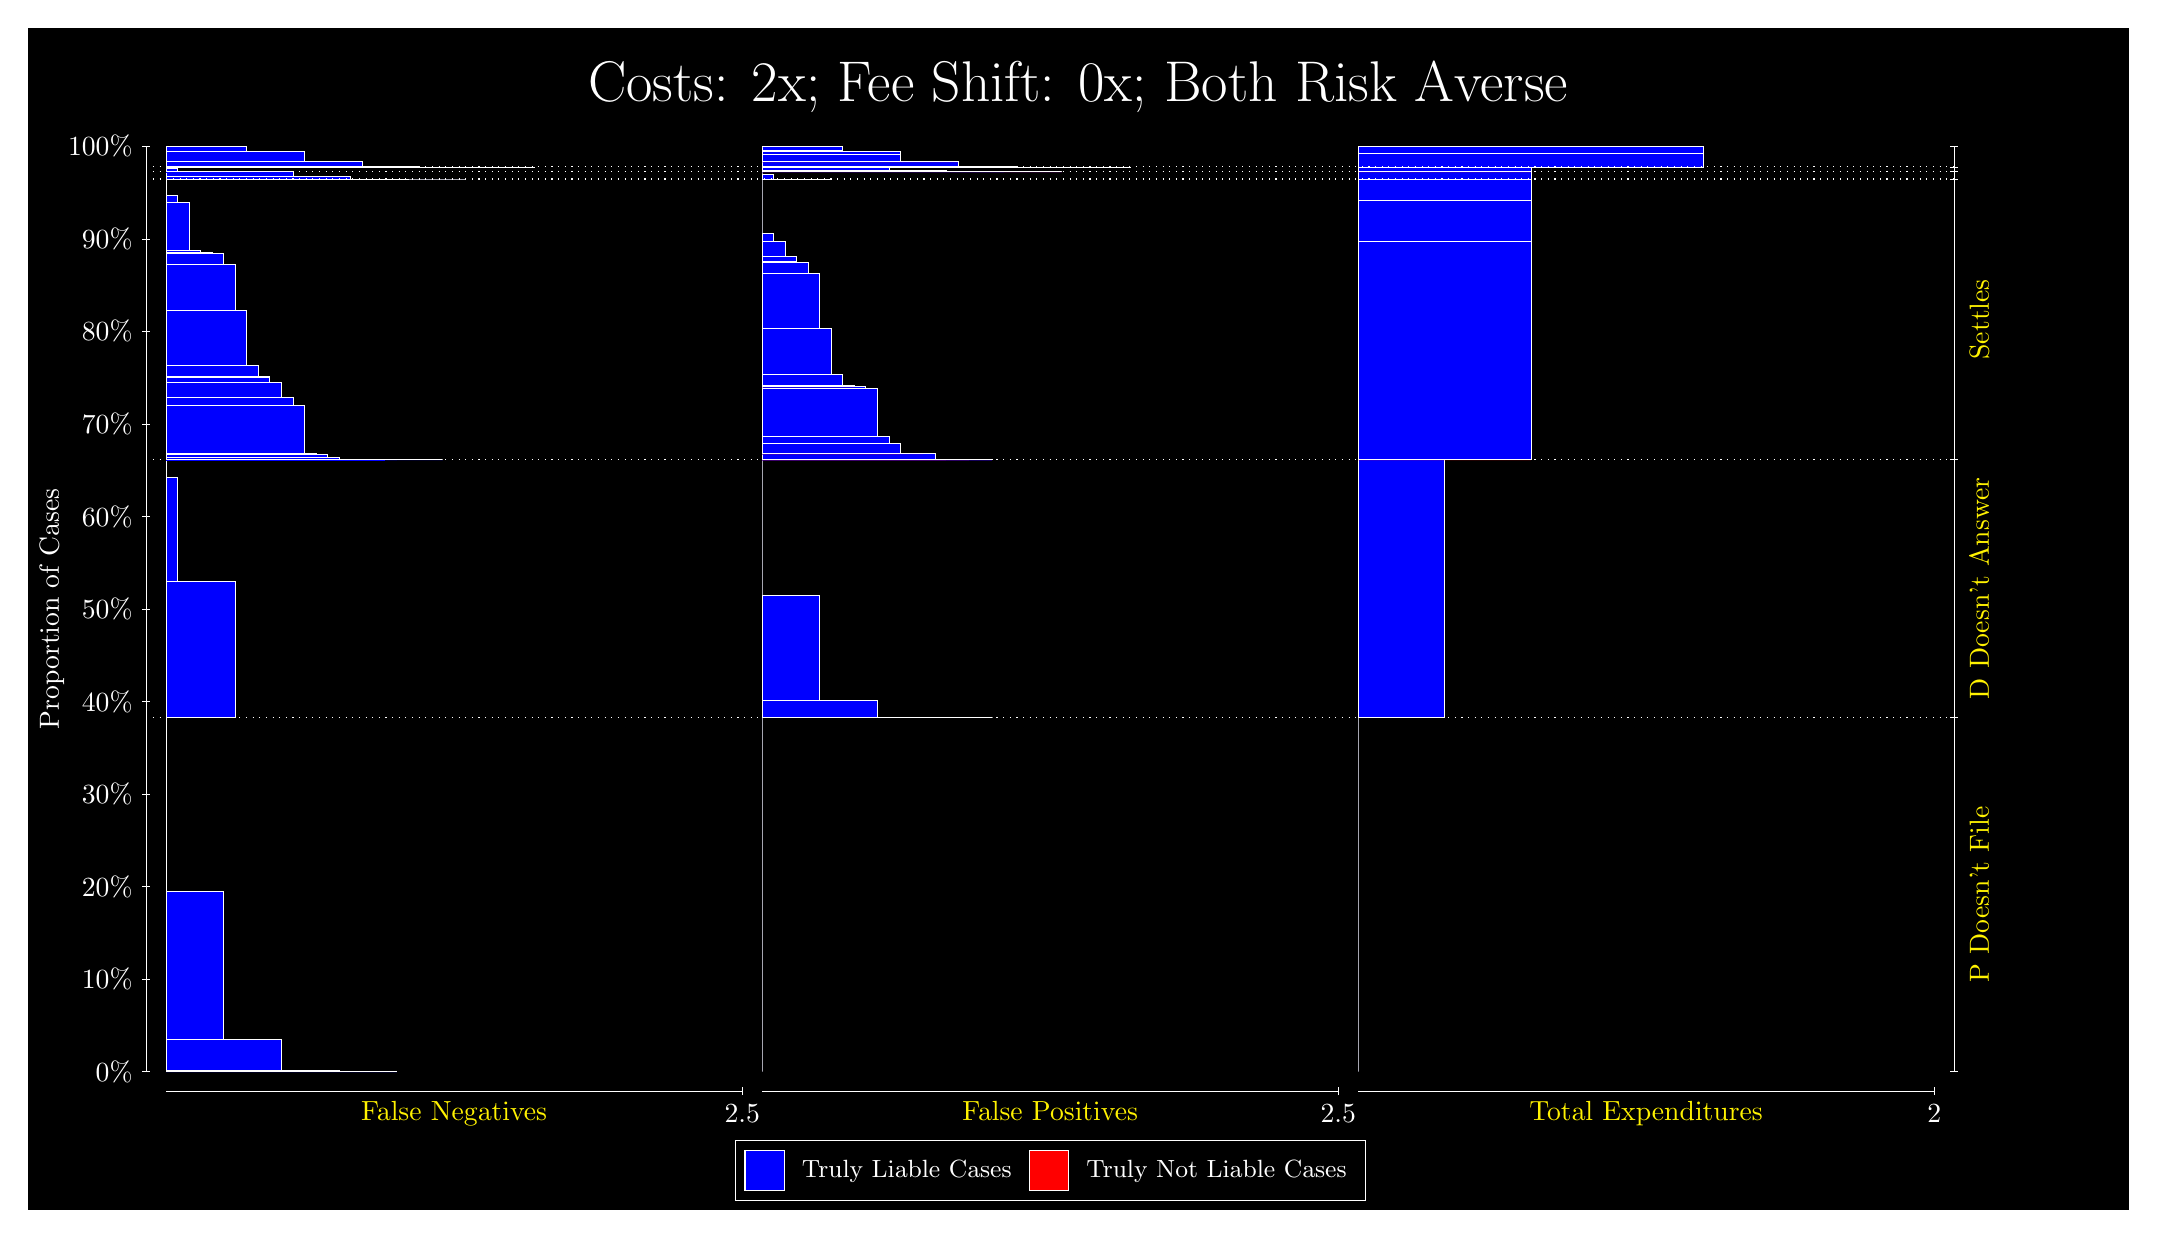
\begin{tikzpicture}
\draw[fill=black] (0,0) rectangle (26.667,15);
\draw[text=white] (0,13.5) rectangle (26.667,15) node[midway] {\huge Costs: 2x; Fee Shift: 0x; Both Risk Averse};
\draw[white, very thin] (1.5,1.75) -- (1.5,13.5);
\node[rotate=90, text=white, anchor=center] at (0.3, 7.625) {Proportion of Cases};
\draw[white, very thin] (1.45,1.75) -- (1.55,1.75);
\node[text=white, anchor=east] at (1.45, 1.75) {0\%};
\draw[white, very thin] (1.45,2.925) -- (1.55,2.925);
\node[text=white, anchor=east] at (1.45, 2.925) {10\%};
\draw[white, very thin] (1.45,4.1) -- (1.55,4.1);
\node[text=white, anchor=east] at (1.45, 4.1) {20\%};
\draw[white, very thin] (1.45,5.275) -- (1.55,5.275);
\node[text=white, anchor=east] at (1.45, 5.275) {30\%};
\draw[white, very thin] (1.45,6.45) -- (1.55,6.45);
\node[text=white, anchor=east] at (1.45, 6.45) {40\%};
\draw[white, very thin] (1.45,7.625) -- (1.55,7.625);
\node[text=white, anchor=east] at (1.45, 7.625) {50\%};
\draw[white, very thin] (1.45,8.8) -- (1.55,8.8);
\node[text=white, anchor=east] at (1.45, 8.8) {60\%};
\draw[white, very thin] (1.45,9.975) -- (1.55,9.975);
\node[text=white, anchor=east] at (1.45, 9.975) {70\%};
\draw[white, very thin] (1.45,11.15) -- (1.55,11.15);
\node[text=white, anchor=east] at (1.45, 11.15) {80\%};
\draw[white, very thin] (1.45,12.325) -- (1.55,12.325);
\node[text=white, anchor=east] at (1.45, 12.325) {90\%};
\draw[white, very thin] (1.45,13.5) -- (1.55,13.5);
\node[text=white, anchor=east] at (1.45, 13.5) {100\%};

\draw[white, very thin] (24.457,1.75) -- (24.457,13.5);
\draw[white, very thin] (24.407,1.75) -- (24.507,1.75);
\node[anchor=west] at (24.407, 1.75) {};
\draw[white, very thin] (24.407,6.2518) -- (24.507,6.2518);
\node[anchor=west] at (24.407, 6.2518) {};
\draw[white, very thin] (24.407,9.5196) -- (24.507,9.5196);
\node[anchor=west] at (24.407, 9.5196) {};
\draw[white, very thin] (24.407,13.085) -- (24.507,13.085);
\node[anchor=west] at (24.407, 13.085) {};
\draw[white, very thin] (24.407,13.179) -- (24.507,13.179);
\node[anchor=west] at (24.407, 13.179) {};
\draw[white, very thin] (24.407,13.24) -- (24.507,13.24);
\node[anchor=west] at (24.407, 13.24) {};
\draw[white, very thin] (24.407,13.5) -- (24.507,13.5);
\node[anchor=west] at (24.407, 13.5) {};

\draw[white, very thin, fill=blue] (1.75,1.75) rectangle (4.6775,1.7501);
\draw[white, very thin, fill=blue] (1.75,1.7501) rectangle (3.9457,1.7632);
\draw[white, very thin, fill=blue] (1.75,1.7632) rectangle (3.2138,2.1589);
\draw[white, very thin, fill=blue] (1.75,2.1589) rectangle (2.4819,4.0358);
\draw[white, very thin, fill=red] (1.75,4.0358) rectangle (1.75,4.0358);
\draw[white, very thin, fill=blue] (1.75,4.0358) rectangle (1.75,6.2518);
\draw[white, very thin, fill=blue] (1.75,6.2518) rectangle (2.6283,7.9751);
\draw[white, very thin, fill=blue] (1.75,7.9751) rectangle (1.8964,9.3029);
\draw[white, very thin, fill=red] (1.75,9.3029) rectangle (1.75,9.3029);
\draw[white, very thin, fill=blue] (1.75,9.3029) rectangle (1.75,9.5196);
\draw[white, very thin, fill=blue] (1.75,9.5196) rectangle (5.2631,9.5196);
\draw[white, very thin, fill=blue] (1.75,9.5196) rectangle (4.6775,9.5197);
\draw[white, very thin, fill=blue] (1.75,9.5197) rectangle (4.5312,9.5208);
\draw[white, very thin, fill=blue] (1.75,9.5208) rectangle (4.3848,9.5208);
\draw[white, very thin, fill=blue] (1.75,9.5208) rectangle (4.092,9.5211);
\draw[white, very thin, fill=blue] (1.75,9.5211) rectangle (3.9457,9.5462);
\draw[white, very thin, fill=blue] (1.75,9.5462) rectangle (3.7993,9.5916);
\draw[white, very thin, fill=blue] (1.75,9.5916) rectangle (3.6529,9.5981);
\draw[white, very thin, fill=blue] (1.75,9.5981) rectangle (3.5065,10.206);
\draw[white, very thin, fill=blue] (1.75,10.206) rectangle (3.3602,10.312);
\draw[white, very thin, fill=blue] (1.75,10.312) rectangle (3.2138,10.5);
\draw[white, very thin, fill=blue] (1.75,10.5) rectangle (3.0674,10.567);
\draw[white, very thin, fill=blue] (1.75,10.567) rectangle (3.0674,10.577);
\draw[white, very thin, fill=blue] (1.75,10.577) rectangle (2.921,10.713);
\draw[white, very thin, fill=blue] (1.75,10.713) rectangle (2.7746,11.414);
\draw[white, very thin, fill=blue] (1.75,11.414) rectangle (2.6283,11.997);
\draw[white, very thin, fill=blue] (1.75,11.997) rectangle (2.4819,12.141);
\draw[white, very thin, fill=blue] (1.75,12.141) rectangle (2.3355,12.157);
\draw[white, very thin, fill=blue] (1.75,12.157) rectangle (2.3355,12.157);
\draw[white, very thin, fill=blue] (1.75,12.157) rectangle (2.1891,12.181);
\draw[white, very thin, fill=blue] (1.75,12.181) rectangle (2.0428,12.791);
\draw[white, very thin, fill=blue] (1.75,12.791) rectangle (1.8964,12.879);
\draw[white, very thin, fill=red] (1.75,12.879) rectangle (1.75,12.879);
\draw[white, very thin, fill=blue] (1.75,12.879) rectangle (1.75,13.085);
\draw[white, very thin, fill=blue] (1.75,13.085) rectangle (5.5558,13.085);
\draw[white, very thin, fill=blue] (1.75,13.085) rectangle (4.8239,13.086);
\draw[white, very thin, fill=blue] (1.75,13.086) rectangle (4.092,13.12);
\draw[white, very thin, fill=blue] (1.75,13.12) rectangle (3.3602,13.178);
\draw[white, very thin, fill=blue] (1.75,13.178) rectangle (2.6283,13.179);
\draw[white, very thin, fill=red] (1.75,13.179) rectangle (1.75,13.179);
\draw[white, very thin, fill=blue] (1.75,13.179) rectangle (2.6283,13.18);
\draw[white, very thin, fill=blue] (1.75,13.18) rectangle (1.8964,13.217);
\draw[white, very thin, fill=red] (1.75,13.217) rectangle (1.75,13.217);
\draw[white, very thin, fill=blue] (1.75,13.217) rectangle (1.75,13.24);
\draw[white, very thin, fill=blue] (1.75,13.24) rectangle (6.4341,13.24);
\draw[white, very thin, fill=blue] (1.75,13.24) rectangle (5.7022,13.24);
\draw[white, very thin, fill=blue] (1.75,13.24) rectangle (4.9703,13.244);
\draw[white, very thin, fill=blue] (1.75,13.244) rectangle (4.2384,13.304);
\draw[white, very thin, fill=blue] (1.75,13.304) rectangle (3.5065,13.435);
\draw[white, very thin, fill=blue] (1.75,13.435) rectangle (2.7746,13.496);
\draw[white, very thin, fill=blue] (1.75,13.496) rectangle (2.0428,13.5);
\draw[white, very thin, fill=red] (1.75,13.5) rectangle (1.75,13.5);
\draw[white, very thin, fill=blue] (1.75,13.5) rectangle (1.75,13.5);
\draw[white, very thin, fill=red] (9.3189,1.75) rectangle (9.3189,1.75);
\draw[white, very thin, fill=blue] (9.3189,1.75) rectangle (9.3189,6.2518);
\draw[white, very thin, fill=red] (9.3189,6.2518) rectangle (12.246,6.2518);
\draw[white, very thin, fill=blue] (9.3189,6.2518) rectangle (12.246,6.2518);
\draw[white, very thin, fill=blue] (9.3189,6.2518) rectangle (11.515,6.2527);
\draw[white, very thin, fill=blue] (9.3189,6.2527) rectangle (10.783,6.4685);
\draw[white, very thin, fill=blue] (9.3189,6.4685) rectangle (10.051,7.7963);
\draw[white, very thin, fill=blue] (9.3189,7.7963) rectangle (9.3189,9.5196);
\draw[white, very thin, fill=red] (9.3189,9.5196) rectangle (12.246,9.5196);
\draw[white, very thin, fill=blue] (9.3189,9.5196) rectangle (12.246,9.5198);
\draw[white, very thin, fill=red] (9.3189,9.5198) rectangle (11.954,9.5198);
\draw[white, very thin, fill=blue] (9.3189,9.5198) rectangle (11.954,9.5198);
\draw[white, very thin, fill=red] (9.3189,9.5198) rectangle (11.661,9.5198);
\draw[white, very thin, fill=blue] (9.3189,9.5198) rectangle (11.661,9.5199);
\draw[white, very thin, fill=blue] (9.3189,9.5199) rectangle (11.515,9.5957);
\draw[white, very thin, fill=red] (9.3189,9.5957) rectangle (11.368,9.5957);
\draw[white, very thin, fill=blue] (9.3189,9.5957) rectangle (11.368,9.5959);
\draw[white, very thin, fill=blue] (9.3189,9.5959) rectangle (11.222,9.5959);
\draw[white, very thin, fill=red] (9.3189,9.5959) rectangle (11.075,9.5959);
\draw[white, very thin, fill=blue] (9.3189,9.5959) rectangle (11.075,9.7263);
\draw[white, very thin, fill=blue] (9.3189,9.7263) rectangle (10.929,9.8143);
\draw[white, very thin, fill=blue] (9.3189,9.8143) rectangle (10.783,10.424);
\draw[white, very thin, fill=blue] (9.3189,10.424) rectangle (10.636,10.448);
\draw[white, very thin, fill=red] (9.3189,10.448) rectangle (10.49,10.448);
\draw[white, very thin, fill=blue] (9.3189,10.448) rectangle (10.49,10.448);
\draw[white, very thin, fill=blue] (9.3189,10.448) rectangle (10.49,10.464);
\draw[white, very thin, fill=blue] (9.3189,10.464) rectangle (10.344,10.608);
\draw[white, very thin, fill=blue] (9.3189,10.608) rectangle (10.197,11.191);
\draw[white, very thin, fill=blue] (9.3189,11.191) rectangle (10.051,11.892);
\draw[white, very thin, fill=blue] (9.3189,11.892) rectangle (9.9044,12.028);
\draw[white, very thin, fill=blue] (9.3189,12.028) rectangle (9.758,12.038);
\draw[white, very thin, fill=blue] (9.3189,12.038) rectangle (9.758,12.105);
\draw[white, very thin, fill=blue] (9.3189,12.105) rectangle (9.6116,12.293);
\draw[white, very thin, fill=blue] (9.3189,12.293) rectangle (9.4652,12.399);
\draw[white, very thin, fill=blue] (9.3189,12.399) rectangle (9.3189,13.085);
\draw[white, very thin, fill=red] (9.3189,13.085) rectangle (10.197,13.085);
\draw[white, very thin, fill=blue] (9.3189,13.085) rectangle (10.197,13.087);
\draw[white, very thin, fill=blue] (9.3189,13.087) rectangle (9.4652,13.144);
\draw[white, very thin, fill=blue] (9.3189,13.144) rectangle (9.3189,13.179);
\draw[white, very thin, fill=red] (9.3189,13.179) rectangle (13.125,13.179);
\draw[white, very thin, fill=blue] (9.3189,13.179) rectangle (13.125,13.179);
\draw[white, very thin, fill=blue] (9.3189,13.179) rectangle (12.393,13.179);
\draw[white, very thin, fill=blue] (9.3189,13.179) rectangle (11.661,13.202);
\draw[white, very thin, fill=blue] (9.3189,13.202) rectangle (10.929,13.239);
\draw[white, very thin, fill=blue] (9.3189,13.239) rectangle (10.197,13.24);
\draw[white, very thin, fill=red] (9.3189,13.24) rectangle (14.003,13.24);
\draw[white, very thin, fill=blue] (9.3189,13.24) rectangle (14.003,13.24);
\draw[white, very thin, fill=red] (9.3189,13.24) rectangle (13.271,13.24);
\draw[white, very thin, fill=blue] (9.3189,13.24) rectangle (13.271,13.24);
\draw[white, very thin, fill=red] (9.3189,13.24) rectangle (12.539,13.24);
\draw[white, very thin, fill=blue] (9.3189,13.24) rectangle (12.539,13.244);
\draw[white, very thin, fill=blue] (9.3189,13.244) rectangle (11.807,13.304);
\draw[white, very thin, fill=red] (9.3189,13.304) rectangle (11.807,13.304);
\draw[white, very thin, fill=blue] (9.3189,13.304) rectangle (11.807,13.304);
\draw[white, very thin, fill=blue] (9.3189,13.304) rectangle (11.075,13.397);
\draw[white, very thin, fill=red] (9.3189,13.397) rectangle (11.075,13.397);
\draw[white, very thin, fill=blue] (9.3189,13.397) rectangle (11.075,13.435);
\draw[white, very thin, fill=blue] (9.3189,13.435) rectangle (10.344,13.451);
\draw[white, very thin, fill=blue] (9.3189,13.451) rectangle (10.344,13.496);
\draw[white, very thin, fill=blue] (9.3189,13.496) rectangle (9.6116,13.496);
\draw[white, very thin, fill=blue] (9.3189,13.496) rectangle (9.6116,13.5);
\draw[white, very thin, fill=blue] (9.3189,13.5) rectangle (9.3189,13.5);
\draw[white, very thin, fill=red] (16.888,1.75) rectangle (16.888,1.75);
\draw[white, very thin, fill=blue] (16.888,1.75) rectangle (16.888,6.2518);
\draw[white, very thin, fill=red] (16.888,6.2518) rectangle (17.986,6.2518);
\draw[white, very thin, fill=blue] (16.888,6.2518) rectangle (17.986,9.5196);
\draw[white, very thin, fill=red] (16.888,9.5196) rectangle (19.083,9.5196);
\draw[white, very thin, fill=blue] (16.888,9.5196) rectangle (19.083,12.292);
\draw[white, very thin, fill=red] (16.888,12.292) rectangle (19.083,12.292);
\draw[white, very thin, fill=blue] (16.888,12.292) rectangle (19.083,12.82);
\draw[white, very thin, fill=red] (16.888,12.82) rectangle (19.083,12.82);
\draw[white, very thin, fill=blue] (16.888,12.82) rectangle (19.083,13.085);
\draw[white, very thin, fill=red] (16.888,13.085) rectangle (19.083,13.085);
\draw[white, very thin, fill=blue] (16.888,13.085) rectangle (19.083,13.179);
\draw[white, very thin, fill=red] (16.888,13.179) rectangle (19.083,13.179);
\draw[white, very thin, fill=blue] (16.888,13.179) rectangle (19.083,13.24);
\draw[white, very thin, fill=red] (16.888,13.24) rectangle (21.279,13.24);
\draw[white, very thin, fill=blue] (16.888,13.24) rectangle (21.279,13.412);
\draw[white, very thin, fill=red] (16.888,13.412) rectangle (21.279,13.412);
\draw[white, very thin, fill=blue] (16.888,13.412) rectangle (21.279,13.5);
\draw[white, dotted] (1.5,6.2518) -- (24.457,6.2518);
\draw[white, dotted] (1.5,9.5196) -- (24.457,9.5196);
\draw[white, dotted] (1.5,13.085) -- (24.457,13.085);
\draw[white, dotted] (1.5,13.179) -- (24.457,13.179);
\draw[white, dotted] (1.5,13.24) -- (24.457,13.24);
\draw[white, very thin] (1.75,1.5) -- (9.0689,1.5);
\node[text=yellow, anchor=north] at (5.4094, 1.5) {False Negatives};
\draw[white, very thin] (9.0689,1.45) -- (9.0689,1.55);
\node[text=white, anchor=north] at (9.0689, 1.45) {2.5};

\draw[white, very thin] (9.3189,1.5) -- (16.638,1.5);
\node[text=yellow, anchor=north] at (12.978, 1.5) {False Positives};
\draw[white, very thin] (16.638,1.45) -- (16.638,1.55);
\node[text=white, anchor=north] at (16.638, 1.45) {2.5};

\draw[white, very thin] (16.888,1.5) -- (24.207,1.5);
\node[text=yellow, anchor=north] at (20.547, 1.5) {Total Expenditures};
\draw[white, very thin] (24.207,1.45) -- (24.207,1.55);
\node[text=white, anchor=north] at (24.207, 1.45) {2};

\node[text=yellow, centered, rotate=90] at (24.777, 4.0009) {P Doesn't File};
\node[text=yellow, centered, rotate=90] at (24.777, 7.8857) {D Doesn't Answer};
\node[text=yellow, centered, rotate=90] at (24.777, 11.303) {Settles};




\draw (12.978300999999998,1.5) node[draw=none] (baseCoordinate) {};
\begin{scope}[align=center]
        \matrix[scale=0.5, draw=white, below=0.5cm of baseCoordinate, nodes={draw}, column sep=0.1cm]{
            \node[rectangle, draw, minimum width=0.5cm, minimum height=0.5cm, fill=blue] {}; &
            \node[draw=none, font=\small, text=white] (B) {Truly Liable Cases}; &
            \node[rectangle, draw, minimum width=0.5cm, minimum height=0.5cm, fill=red] {}; &
            \node[draw=none, font=\small, text=white] (B) {Truly Not Liable Cases}; \\
            };
\end{scope}

\end{tikzpicture}
\end{document}